\subsection{Energiekalibration}
\begin{itemize}
	\item Spektrum geplottet, Counts gegen Channel
	\item Errorbars?
	\item Peaks finden lassen, Peaks markiert
	\item Literaturwerte Energien rausgesucht mit mind. 1\% Emissionswahrscheinlichkeit (Quelle %http://www.nucleide.org/DDEP_WG/Nuclides/Eu-152_tables.pdf 2019-12-11, 22:35)
	\item Spektrallinien $E$ normiert mit dem größten Wert der Energie: $\frac{E}{max(E)}$
	\item Channel normiert mit dem letzten Peak $\frac{channel}{max(channel)}$
	\item Daten mit normierter x-Achse geplottet: norm(E)-0-Diagramm, norm(channel)-Count-Diagramm
	\item Nicht vorhandene Spektrallinien aus E und doppelte aus Peaks entfernt
	\item Peak-Channel gegen Energien geplottet, Fit:
\end{itemize}
\begin{equation*}
	E = m \cdot \text{Channel} + n
\end{equation*}
\begin{align*}
	m = \SI{0.20726(4)}{\kilo \electronvolt \per Channel} && n = \SI{-1.22(17)}{\kilo \electronvolt}
\end{align*}

\begin{figure}[h!]
  \centering
  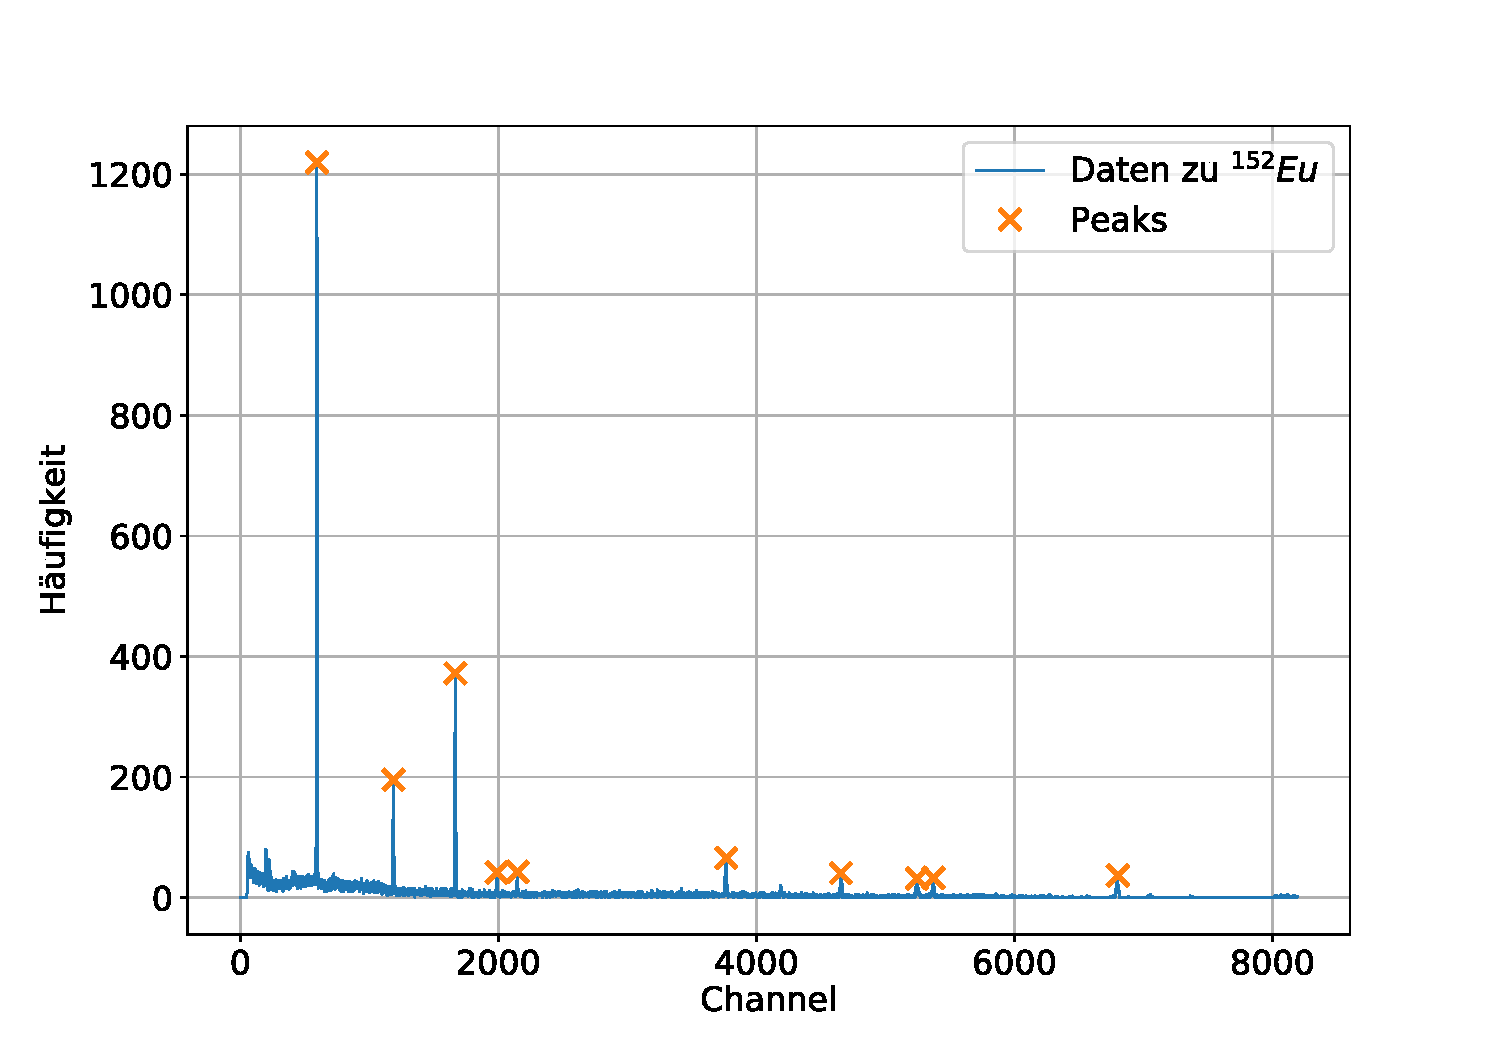
\includegraphics[width=0.8\textwidth]{content/images/spektrum_europium.pdf}
  \caption{Das aufgenommene Spektrum von $^{152}Eu$ mit eingezeichneten Peaks.}
  \label{fig:eu_spect}
\end{figure}

\begin{figure}[h!]
  \centering
  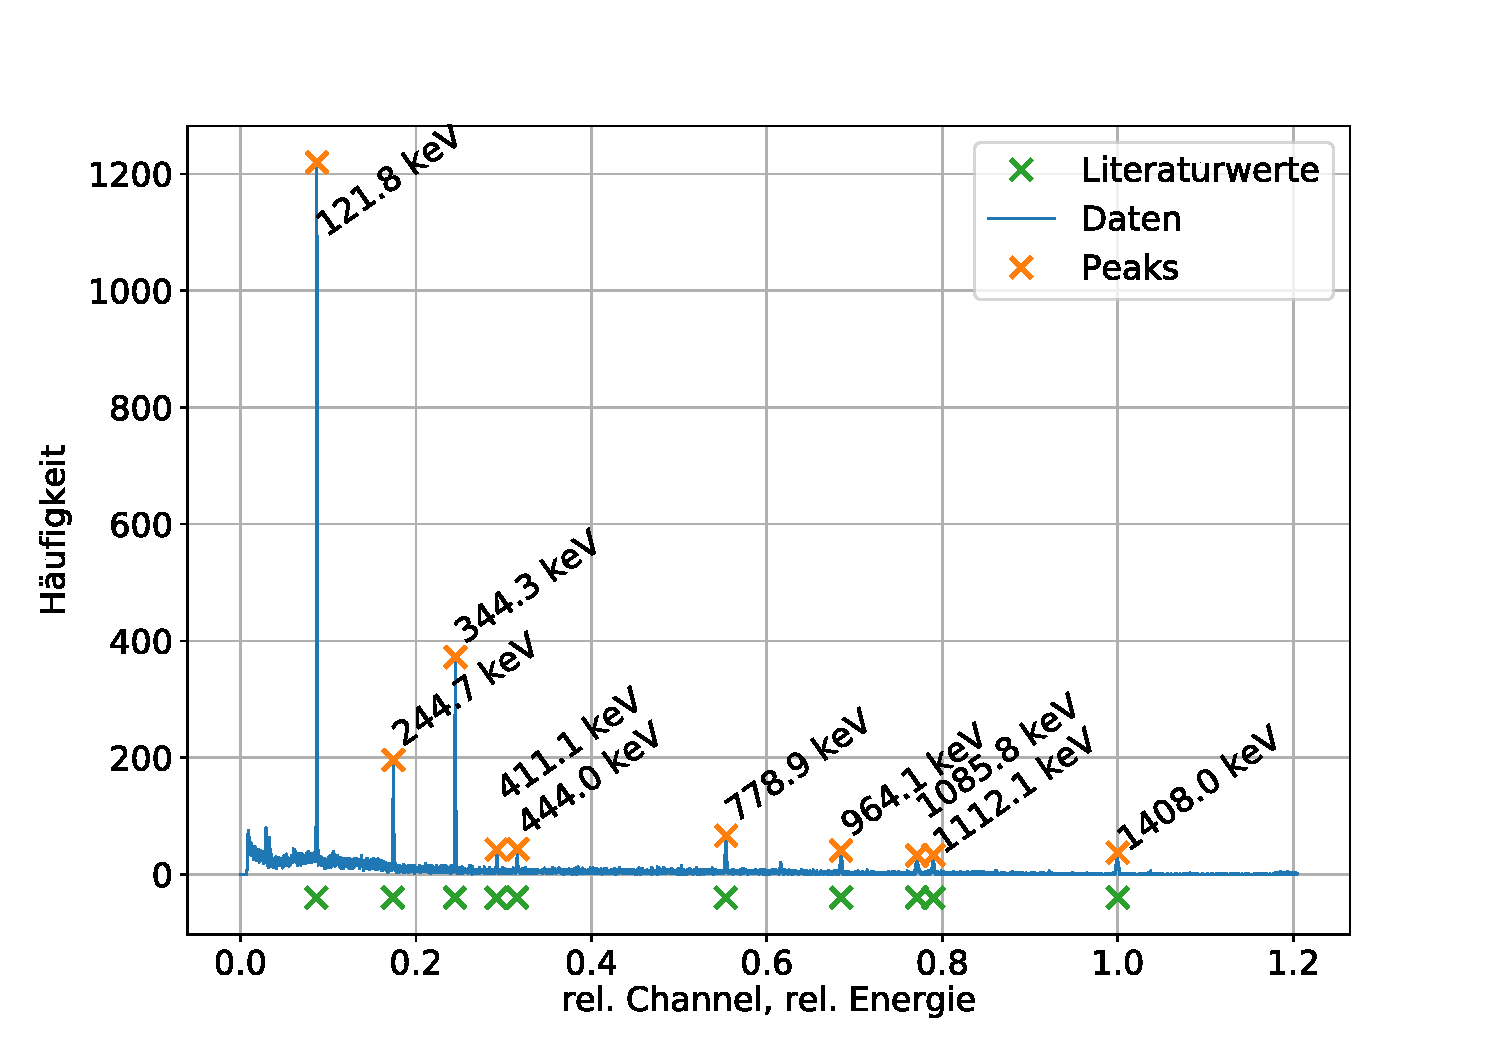
\includegraphics[width=0.8\textwidth]{content/images/spektrum_europium_kali.pdf}
  \caption{Das aufgenommene Spektrum von $^{152}Eu$ mit eingezeichneten Peaks und den zugehörigen Literaturwerten nach %\cite{eu_energie}
  .}
  \label{fig:eu_spect_kali}
\end{figure}

\begin{figure}[h!]
  \centering
  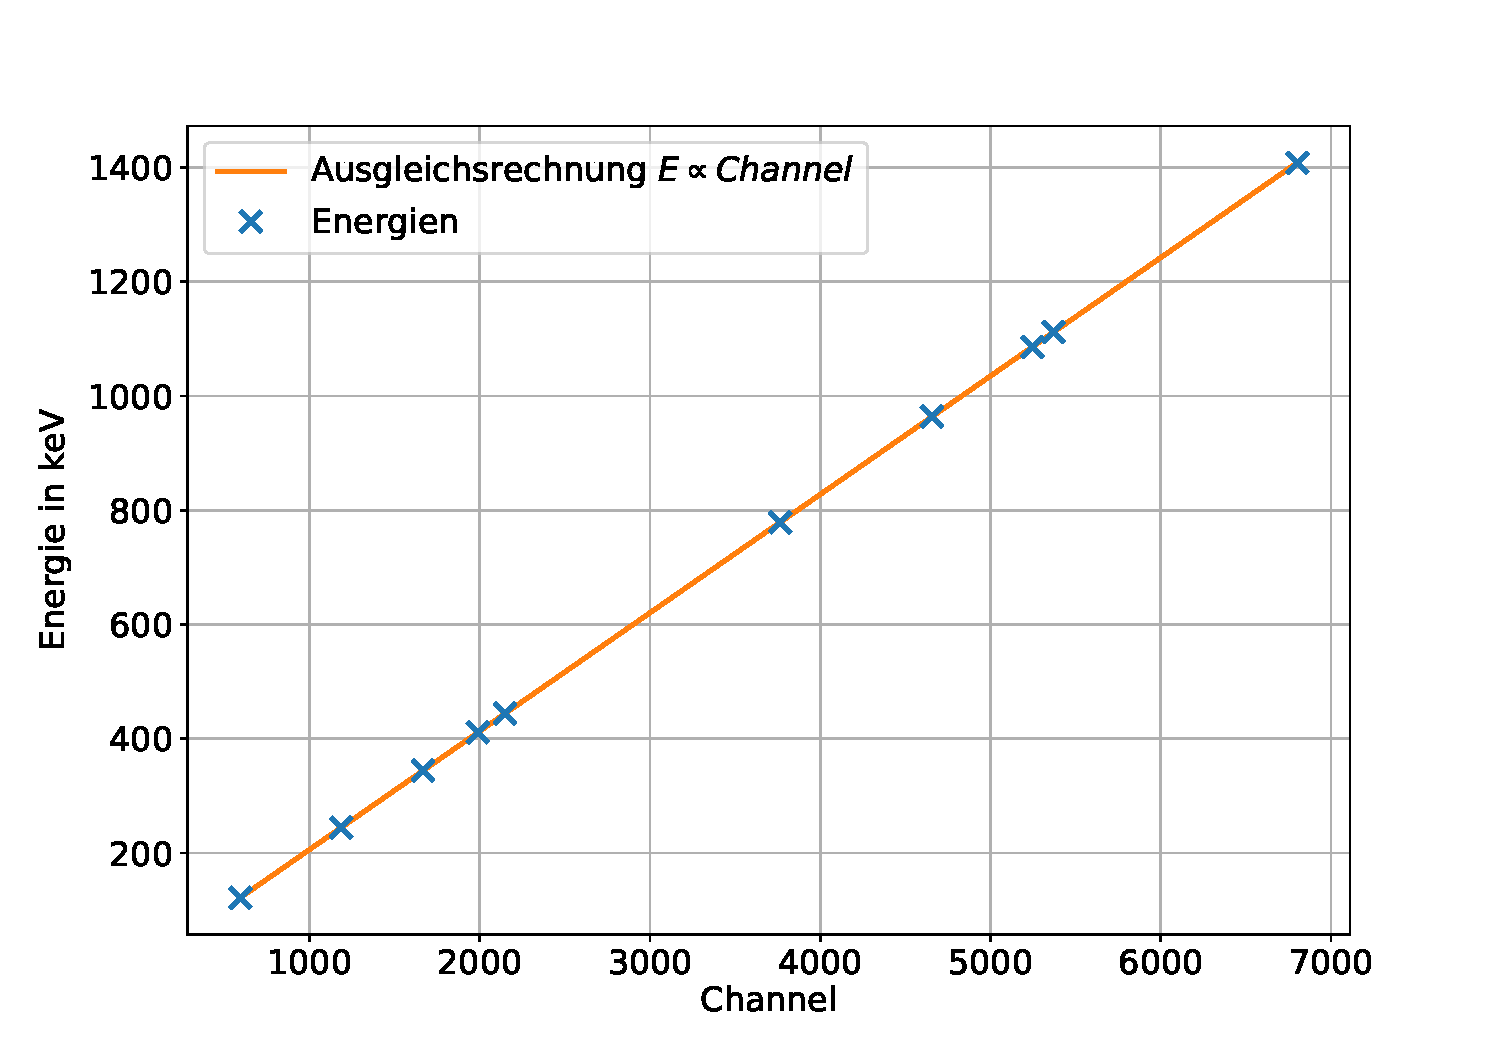
\includegraphics[width=0.8\textwidth]{content/images/kalibration.pdf}
  \caption{Ausgleichsrechnung zur Kalibration mithilfe des $^{152}Eu$-Spektrums.}
  \label{fig:kali}
\end{figure}


\subsection{Vollenergienachweiswahrscheinlichkeit}
mit $t = \SI{605484000 (54000)}{s}$
und $T_{\sfrac{1}{2}} = \SI{426.7 (5) e+06}{s}$ %http://www.nucleide.org/Laraweb/index.php 2019-12-12 18:40
\begin{equation*}
	A = A_{0} \exp{\left( - \frac{\ln{(2))}}{T_{\sfrac{1}{2}}} t \right)} = \SI{1545 (29)}{\per \second}
\end{equation*}
mit $r=\SI{22.5e-03}{m}$
und $h = \SI{65e-03}{m}$
\begin{align*}
	\frac{r}{h} = \tan{( \varphi / 2 )} \Leftrightarrow \varphi = 2 \arctan{(\frac{r}{h})} \\
	\Omega = 4 \pi \sin^2{\frac{\varphi}{2 \cdot 4}} = 4 \pi \sin^2{ \left( \frac{1}{4} \arctan{(r/h)} \right)}
\end{align*}
